\documentclass[11pt, ngerman, fleqn, DIV=15, headinclude, BCOR=2cm]{scrreprt}

\usepackage{../../header}

\usepackage{placeins}
%\usepackage[maxfloats=50]{morefloats}

\usepackage{csquotes}

\usepackage{tikz}
\usetikzlibrary{chains}
\usetikzlibrary{shapes.geometric}

\tikzset{device/.style={
                rectangle,
                minimum size=6mm,
                draw=black
            },
            monitor/.style={
                rectangle,
                rounded corners=2mm,
                minimum size=6mm,
                draw=black
            },
        }

\usepackage{pgfplots}
\pgfplotsset{
    compat=1.9,
    width=0.8\linewidth,
    xticklabel style={/pgf/number format/use comma},
    yticklabel style={/pgf/number format/use comma},
}
\usepgfplotslibrary{polar}

\usepgfplotslibrary{external}
\tikzexternalize[mode=list and make]
\tikzsetexternalprefix{Abbildung-}

\DeclareSIUnit{\skt}{SKT}

\usepackage{booktabs}

\usepackage{subcaption}

\hypersetup{
    pdftitle=
}

\newcommand{\plotwidth}{0.8\linewidth}

\subject{Praktikumsprotokoll}
\title{Nukleare Elektronik und Lebensdauermessung}
\subtitle{Versuch P525 -- Universität Bonn}
\author{
	Frederike Schrödel \\
	\small{\href{mailto:fschroedel@gmx.de}{fschroedel@gmx.de}}
	\and
	Simon Schlepphorst \\
	\small{\href{mailto:s2@uni-bonn.de}{s2@uni-bonn.de}}
}

\date{2015-12-08 bis 12-09}

\publishers{Tutor: Philipp Hoffmeister
}

\begin{document}

\maketitle

\begin{abstract}
	Das Versuchsziel ist die Lebensdauer des angeregten $5/2^+$
        Zustandes einer $^{133}\text{Cs}$ Quelle zu bestimmen.
\end{abstract}


\tableofcontents

\chapter{Theorie}

% TODO

\section{Szintillationsdetektor}

Mit einem Szintillationsdetektor lassen sich Intensität und Energie von
ionisierender Strahlung messen.
Er besteht aus einem Szintillator und einem Photomultiplier.
Der Szintillator ist ein dotierter Einkristall, der von energiereicher
Strahlung zum Fluoreszieren angeregt werden kann und hinreichend
durchlässig für das von ihm emittierte Licht ist.

Innerhalb des vor Lichteinfall geschützten Szintillators entstehen durch
ionisierende Strahlung Lichtblitze. 
% FIXME Sinn?
Diese entstehen dadurch, dass die Strahlung Atome durch die
Effekt~\ref{sec:WW-strahlung-Materie} anregt, welche entweder direkt
wieder rekombinieren und Photonen aussenden oder über Stöße vorher einen Teil
ihrer Energie abgeben.
Somit ist die Intensität dieser Blitze abhängig von der Energie der einfallenden Strahlung.

\subsection{Photomultiplier}

Aufgrund des Photoeffektes werden an der Photokathode des Photomultipliers
Elektronen ausgelöst.

Durch den Aufbau des Photomultipliers kommt es zu einem Lawineneffekt,
welcher die Elektronen vervielfacht und somit eine Detektion erleichtert.
Die Amplitude des so entstanden Strompulses ist somit auch proportional zu der
Energie der Eingangsstrahlung.

\subsection{Energie und Zeitauflösung}

Um mit dieser Art Detektor möglichst gute Auflösungen zu erhalten, greift man
das Signal -- je nachdem ob man die Energie- oder die Zeitauflösung optimieren
will --
an einer Dynode bzw.\ an der Anode des Photomultipliers ab.
Der Vorteil der Dynode für die Energieauflösung liegt dadrin, dass noch keine
Sättigung herrscht. Hierdurch ist die Proportionalität zwischen Signalhöhe und
Energie nicht beeinträchtigt. Da das Signal allerdings nur sehr langsam
ansteigt, man spricht vom \emph{Slow}-Signal, ist die Zeitauflösung beeinträchtigt.
Deswegen benutzt man hier das sogenannte \emph{Fast}-Signal. Es wird an der Anode
abgegriffen, da dort Sättigung vorliegt, wodurch das Signal schnell ansteigt.
Die Amplitude ist allerdings nicht mehr proportional zur Energie.
Um die Zeitauflösung ermitteln zu können nutzt man eine
Slow-Fast-Koinzidenzschaltung. Man misst bekannte Linien und bestimmt aus den
angepassten Funktionen die Halbwertsbreite.

%TODO für Nukleare elektronik
Für die Zeitkalibrierung nutzt man
am besten ein Isotop, welches einen $\beta^+$-Zerfall besitzt. Dadurch kann
man gewährleisten, dass gleichzeitig zwei Photonen mit bekannter Wellenlänge
von \SI{511}{\kilo\electronvolt} durch die Rekombination von Elektron und
Positron entstehen.

\subsection{Splitter}

% XXX Und wie funktioniert so ein Splitter?

Im Laufe des Versuches wird es nötig sein, dass das Signal aufgeteilt wird,
ohne dabei verformt zu werden. Hierfür nutzt man ein Bauteil, welches
\emph{Splitter}
genannt wird. 

\subsection{Einkanalanalysator}

% FIXME Diskriminator noch nicht eingeführt.

Der \emph{Einkanalanalysator}, auch Single Channel Analyser, kurz \emph{SCA}, genannt ist ein
Bauteil, welches ähnlich eines Diskriminators eine untere, aber auch eine obere
Grenze besitzt. Wenn ein Signal die untere Grenze übersteigt, aber die obere
Grenze nicht erreicht, so sendet der SCA ein digitales Signal aus, sobald das
Signal wider unter die untere Grenze sinkt.

\subsection{Vielkanalanalysator}

Um ein nach Amplituden sortiertes Spektrum zu erhalten, nutzen wir ein MCA.
Dies ist ein Bauteil, welches einkommende Signale nach Amplitude sortiert und
dann den Kanal, welcher der Impulshöhe entspricht, hoch setzt. So erhalten wir ein
Histogramm. Der MCA ist aus mehreren SCAs aufgebaut.

\subsection{Constant Fraction Diskriminator}

Ein CFD ist ein Diskriminator und somit in der Lage ein analoges
Eingangsignal in ein digitales Ausgangssignal umzuwandeln, wenn ein Signal einen
bestimmten Wert übersteigt.
Der Constant Fraction Diskriminator ist allerdings auch in der Lage Signale
verschiedener Größe zu detektieren, sofern sie die selbe Form haben, da diese
dann die gleiche Anstiegszeit haben. Das digitale Signal wird abgegeben, sobald
das analoge Signal einen bestimmten Bruchteil seiner Amplitude erreicht.

\subsection{Verstärker}

Ein Verstärker hat, wie der Name schon sagt, die Aufgabe ein Signal zu
verstärken. Man nutzt meist einen Vor- und einen Hauptverstärker um zu
gewährleisten dass die Verstärkung linear ist. 

\subsection{Delays}

Delays sollen die elektrischen Signale verzögern. Da die Länge eines Kabels
proportional zu dessen Verzögerung ist, kann man ein Kabel mit entsprechender
Länge nutzten um eine bestimmte Verzögerung zu erhalten.

\subsection{Koinzidenzeinheit}

Mit der Koinzidenzeinheit lässt sich überprüfen, ob zwei Signale zeitnah
nacheinander auftreffen. Hierzu werden die Eingangssignale über ein logisches
\textsc{and} miteinander verknüpft und im Falle eines Überlapps ein Ausgangssignal
ausgegeben. Dadurch wird aber direkt die Zeitauflösung auf die doppelte
Impulslänge begrenzt.

\subsection{Zeit-Amplituden-Wandler}

Der Zeit-Amplituden-Wandler (time-to-amplitude-converter oder auch TAC) soll
aus der zeitlichen Differenz zweier Signale ein Signal erstellen, welches
in der Amplitude proportional zu der Dauer des Eingangssignals ist. Das lässt
sich beispielsweise dadurch realisieren, dass durch Eintreffen des ersten
Signals ein Kondensator mit einer Konstantstromquelle
aufgeladen wird. Der Ladevorgang wird beendet sobald das zweite Signal
eintrifft. Bei dem Entladen ist das resultierende Signal ist in der Höhe
proportional zu der Zeitdifferenz.

\section{Aufbau zur Zerfallszeitmessung}

Um Zerfallszeiten zu messen, nutzen wir eine Fast-Slow-Koinzidenzschaltung, da
wir sowohl eine gute Zeit- als auch Energieauflösung benötigen. Die Schaltung
sieht dabei wie folgt aus: 
Zwei Detektoren sind so ausgerichtet, dass sie sich gegenüber stehen und die
Probe im selben Abstand zwischen ihnen steht. An die Detektoren wird je ein
Photomultiplier angeschlossen. Die Slow-Ausgänge werden genutzt um die
Koinzidenz von Ereignissen zu überprüfen. Hierzu schneidet man mit dem SCA die
Energiebereiche aus, die verglichen werden sollen. Die beiden Signale aus den
SCAs werden in eine Koinzidenzeinheit geführt und wenn diese ein Signal
produziert, so wird das Signal aus der Fast-Schaltung genutzt; es dient also
als Trigger. Die Fast-Schaltung beginnt am Fast-Ausgang des Photomultipliers.
Von da aus gehen die Signale durch CFDs. Das Signal der einen Seite dient als
Startsignal des TAC, das andere als Stopsignal. Von dort aus wird die so
modellierte Amplitude von einen MCA in ein Histogram gespeichert, sofern im
Slow-Kreis festgestellt wurde, dass es relevant ist.

% TODO Figure in Text referenzieren.

\begin{figure}[htbp]
    \centering
    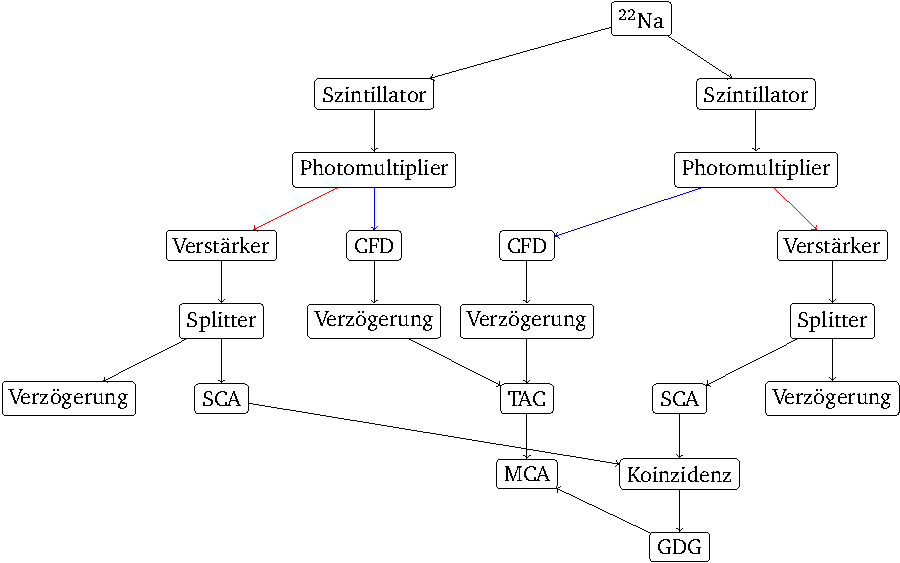
\includegraphics{../Aufbau-crop}
    \caption{%
        %
    }
    \label{fig:}
\end{figure}

\section{Zerfallsschema von $^{22}\text{Na}$ und $^{133}\text{Ba}$}

Das $^{22}\text{Na}$ zerfällt hauptsächlich über einen $\beta^+$-Zerfall in ein
angeregtes $^{22}\text{Ne}$, welches ein Photon mit einer Energie von
\SI{1274,6}{\kilo\electronvolt} emittiert. Das Positron annihiliert mit einem
Elektron und sendet zeitgleich zwei Photonen mit jeweils \SI{511}{\kilo\electronvolt}
aus. Diese fliegen genau in entgegengesetzte Richtung. Deshalb eignet
sich dieser Zerfall hervorragend zur Zeitkalibrierung. 

Für $^{133}\text{Ba}$ ist der wahrscheinlichste Zerfall einer über
Elektroneneinfang, bei dem es in angeregtes $^{133}\text{Cs}$ zerfällt und erst
ein Photon mit \SI{356}{\kilo\electronvolt} abstrahlt. Der entstandene
Zustand ist der angeregte $5/2^+$ Zustand, dessen Lebensdauer wir
bestimmen wollen, bevor er über Abstrahlung eines Photons mit \SI{81}{\kilo\electronvolt}
zerfällt.

% TODO Zerfallsschmata

\chapter{Durchführung}

%TODO

Bei der Durchführung geht es darum den oben beschriebenen Schaltplan Schritt
für Schritt aufzubauen und die einzelnen Bauteile entsprechend zu
kalibrieren. Die folgenden Schritte werden sowohl für die rechte wie auch die
linke Seite des Aufbaus durchgeführt. Zu Beginn nutzen wir das
$^{22}\text{Na}$-Präparat. 

Nachdem die Hochspannung an den Szintillationsspektrometer angelegt wurde, wird
zunächst das Signal aus dem Slow-Ausgang oszilloskopiert.
% TODO Bild
Als nächstes nutzen wir den Splitter um das Signal aus dem Hauptverstärker
reflexionsfrei aufzuteilen. Da das Signal dadurch allerdings schwächer wird,
bleibt der Splitter im gesamten weiteren Verlauf eingebaut. Die eine Hälfte des
Signals geht durch einen Verzögerer in das Oszilloskop, Kanal~1, während das zweite Signal erst
durch einen SCA läuft.
% TODO 
Auf dem Oszilloskop identifizieren wir die deutlichste Linie als die \SI{511}{\kilo\electronvolt}
Linie und versuchen diese über die Verstärkung auf \SIrange{3}{4}{\volt}
einzustellen. Als nächstes verzögern wir das Analogsignal, damit es von dem
Digitalsignal des SCA überdeckt wird.

Nun wird das Signal aus dem Hauptverstärker und das SCA-Signal in den MCA
gegeben und Datensätze aufgenommen. Wir wählen die Verstärkung so, dass die
\SI{511}{\kilo\electronvolt}-Linie sich am rechten Spektrumsrand befindet.
Außerdem muss die \SI{81}{\kilo\electronvolt}-Linie des $^{133}\text{Cs}$ in dem Spektrum
auftauchen.

Nun werden die Einkanalfenster auf \SI{511}{\kilo\electronvolt}
eingestellt. Dafür stellt man die obere und die untere Grenze so ein, dass das
Signal gut umschlossen ist. Wenn man beide Seiten eingestellt hat, dann stellen
wir die Koinzidenz her. Hierfür betrachten wir die beiden Signal auf dem
Oszilloskop und verzögern die Signale so, dass sie möglichst gut überlagern. 

Als nächstes stellen wir den Fast-Kreis ein. Als erstes oszilloskopieren wir
das Fast-Signal. Dann stellen wir die Schwelle von dem CFD ein.
Bei dem erstellen der Fast-Koinzidenz ist wichtig zu entscheiden, welches
Signal als Start- und welches als Stop-Signal für den TAC benutzt werden soll.
Im Zweifelsfall kann man hier einen Verzögerer nutzen. Dabei sollte man darauf
achten, dass die Verzögerungseinheiten möglichst klein gewählt werden. 

% zeitlicher abgleich von Fast- und slow signal
%TODO zeiteichung

Um die Lebensdauer des angeregten $5/2^+$ Zustandes der $^{133}\text{Cs}$
Quelle zu bestimmen tauscht man die Quellen und geht bei der Einstellung ebenso
vor. Hierbei stellt man die Einkanalfenster so ein, dass für das Startsignal
des TACs die \SI{356}{\kilo\electronvolt}- und für das Stopsignal
die \SI{81}{\kilo\electronvolt}-Linie dient.

\section{Slow-Koinzidenzkreis einstellen}
%Na-22
%Slow-Kreis

\begin{figure}
	\centering
	\begin{subfigure}{0.49 \textwidth}
		\includegraphics[width=\textwidth]{TEK00007}
		\caption{%
			links
		}
		\label{fig:slow_signal-li}
	\end{subfigure}
	\begin{subfigure}{0.49 \textwidth}
		\includegraphics[width=\textwidth]{TEK00005}
		\caption{%
			rechts
		}
		\label{fig:slow_signal-re}
	\end{subfigure}
	\caption{%
		Signal nach dem Vorverstärker
	}
	\label{fig:slow_signal}
\end{figure}

\begin{figure}
	\centering
	\begin{subfigure}{0.49 \textwidth}
		\includegraphics[width=\textwidth]{TEK00012}
	\end{subfigure}
	\begin{subfigure}{0.49 \textwidth}
		\includegraphics[width=\textwidth]{TEK00013}
	\end{subfigure}
	\caption{%
		Signal nach dem Hauptverstärker
	}
	\label{fig:slow_signal_hv}
\end{figure}

\begin{figure}
	\centering
	\begin{subfigure}{0.49 \textwidth}
		\includegraphics[width=\textwidth]{TEK00014}
		\caption{%
			links
		}
		\label{fig:slow_signal_sca_trig-li}
	\end{subfigure}
	\begin{subfigure}{0.49 \textwidth}
		\includegraphics[width=\textwidth]{TEK00015}
		\caption{%
			rechts
		}
		\label{fig:slow_signal_sca_trig-re}
	\end{subfigure}
	\caption{%
		Signal nach dem Hauptverstärker mit SCA getriggert\\
		GDG ist in beiden Abbildungen gleich eingestellt
	}
	\label{fig:slow_signal_sca_trig}
\end{figure}

\begin{figure}
	\centering
	\begin{subfigure}{0.49 \textwidth}
		\includegraphics[width=\textwidth]{plot_spektrum_li_na_raw}
		\caption{%
			links
		}
		\label{fig:slow_signal_sca_trig-li_plot}
	\end{subfigure}
	\begin{subfigure}{0.49 \textwidth}
		\includegraphics[width=\textwidth]{plot_spektrum_re_na_raw}
		\caption{%
			rechts
		}
		\label{fig:slow_signal_sca_trig-re_plot}
	\end{subfigure}
	\caption{%
		$^{22}\text{Na}$-Spektrum mit grob eingestelltem
		Hauptverstärker
	}
	\label{fig:slow_signal_sca_trig_plot}
\end{figure}

Anschließend haben wir den Hauptverstärker für beide Seiten jeweils so
eingestellt, dass der \SI{511}{\kilo\electronvolt} Peak aus dem
$^{22}\text{Na}$ am rechten Rand des aufgenommen Spektrums liegt und das
$^{133}\text{Ba}$-Spektrum ebenfalls vollständig aufgenommen wird. Dazu haben
wir die Proben mehrmals gewechselt und den Verstärker feinjustiert bis wir die
in Abbildung~\ref{fig:slow_signal_hv_eingestellt_plot} und
Abbildung~\ref{fig:ba_slow_signal_hv_eingestellt_plot} zu sehenden Spektren
erhalten haben.


\begin{figure}
	\centering
	\begin{subfigure}{0.49 \textwidth}
		\includegraphics[width=\textwidth]{TEK00018}
		\caption{%
			links
		}
		\label{fig:slow_signal_hv_eingestellt-li}
	\end{subfigure}
	\begin{subfigure}{0.49 \textwidth}
		\includegraphics[width=\textwidth]{TEK00017}
		\caption{%
			rechts
		}
		\label{fig:slow_signal_hv_eingestellt-re}
	\end{subfigure}
	\caption{%
		Signal nach dem Hauptverstärker mit SCA getriggert\\
		Nach der Spektrenauswahl durch den Verstärker
	}
	\label{fig:slow_signal_hv_eingestellt}
\end{figure}

\begin{figure}
	\centering
	\begin{subfigure}{0.49 \textwidth}
		\includegraphics[width=\textwidth]{plot_spektrum_li_na}
		\caption{%
			links
		}
		\label{fig:slow_hv_eingestellt-li_plot}
	\end{subfigure}
	\begin{subfigure}{0.49 \textwidth}
		\includegraphics[width=\textwidth]{plot_spektrum_re_na}
		\caption{%
			rechts
		}
		\label{fig:slow_hv_eingestellt-re_plot}
	\end{subfigure}
	\caption{%
		$^{22}\text{Na}$-Spektrum mit fertig eingestelltem
		Hauptverstärker
	}
	\label{fig:slow_signal_hv_eingestellt_plot}
\end{figure}


\begin{figure}
	\centering
	\begin{subfigure}{0.49 \textwidth}
		\includegraphics[width=\textwidth]{TEK00019}
		\caption{%
			links
		}
		\label{fig:slow_signal_sca_eingestellt-li}
	\end{subfigure}
	\begin{subfigure}{0.49 \textwidth}
		\includegraphics[width=\textwidth]{TEK00020}
		\caption{%
			rechts
		}
		\label{fig:slow_signal_sca_eingestellt-re}
	\end{subfigure}
	\caption{%
		Signal nach dem Hauptverstärker, Schwellen des SCA auf
		$^{22}\text{Na}$-Spektrum angepasst.
	}
	\label{fig:slow_signal_sca_eingestellt}
\end{figure}

\begin{figure}
	\centering
	\begin{subfigure}{0.49 \textwidth}
		\includegraphics[width=\textwidth]{plot_spektrum_filter_li_Na}
		\caption{%
			links
		}
		\label{fig:slow_sca_eingestellt-li_plot}
	\end{subfigure}
	\begin{subfigure}{0.49 \textwidth}
		\includegraphics[width=\textwidth]{plot_spektrum_filter_re_Na}
		\caption{%
			rechts
		}
		\label{fig:slow_sca_eingestellt-re_plot}
	\end{subfigure}
	\caption{%
		$^{22}\text{Na}$-Spektrum nach Auswahl durch SCA
	}
	\label{fig:slow_signal_sca_eingestellt_plot}
\end{figure}

Durch das Einstellen des SCA haben wir links die Kanäle
\numrange{<< li_Na_lower_channel >>}{<< li_Na_upper_channel >>} und rechts
die Kanäle
\numrange{<< re_Na_lower_channel >>}{<< re_Na_upper_channel >>} ausgewählt.

\begin{figure}
	\centering
	\begin{subfigure}{0.49 \textwidth}
		\includegraphics[width=\textwidth]{TEK00021}
	\end{subfigure}
	\begin{subfigure}{0.49 \textwidth}
		\includegraphics[width=\textwidth]{TEK00022}
	\end{subfigure}
	\caption{%
		Koinzidenz der SCA gegeneinander. Kanal 1 ist der linke
		Detektor, Kanal 2 der rechte.
	}
	\label{fig:slow_signal_sca_koinzidenz}
\end{figure}


%Fast-Kreis

\begin{figure}
	\centering
	\begin{subfigure}{0.49 \textwidth}
		\includegraphics[width=\textwidth]{TEK00027}
		\caption{%
			links
		}
		\label{fig:fast_signal-li}
	\end{subfigure}
	\begin{subfigure}{0.49 \textwidth}
		\includegraphics[width=\textwidth]{TEK00028}
		\caption{%
			rechts
		}
		\label{fig:fast_signal-re}
	\end{subfigure}
	\caption{%
		Fast Pulse vom Photomultiplier. Auf der rechten Seite haben wir
		den recht kurz aufleuchtenden Puls mit dem langsam speichernden
		Oszilloskop nicht getroffen. Er sah aber genauso aus wie links.
	}
	\label{fig:fast_signal}
\end{figure}

\begin{figure}
	\centering
	\begin{subfigure}{0.49 \textwidth}
		\includegraphics[width=\textwidth]{TEK00031}
		\caption{%
			links
		}
		\label{fig:fast_signal_cfd_trig-li}
	\end{subfigure}
	\begin{subfigure}{0.49 \textwidth}
		\includegraphics[width=\textwidth]{TEK00032}
		\caption{%
			rechts
		}
		\label{fig:fast_signal_cfd_trig-re}
	\end{subfigure}
	\caption{%
		Signal nach dem Hauptverstärker mit CFD getriggert
	}
	\label{fig:fast_signal_cfd_trig}
\end{figure}

\begin{figure}
	\centering
	\begin{subfigure}{0.49 \textwidth}
		\includegraphics[width=\textwidth]{plot_spektrum_cfd_li_Na}
		\caption{%
			links
		}
		\label{fig:fast_signal_cfd_plot-li}
	\end{subfigure}
	\begin{subfigure}{0.49 \textwidth}
		\includegraphics[width=\textwidth]{plot_spektrum_cfd_re_Na}
		\caption{%
			rechts
		}
		\label{fig:fast_signal_cfd_plot-re}
	\end{subfigure}
	\caption{%
		$^{22}\text{Na}$-Spektrum nach dem Setzen der CFD Schwellen
	}
	\label{fig:fast_signal_cfd_plot}
\end{figure}

Durch das Einstellen des CFD haben wir links die Kanäle
\numrange{<< li_Na_lower_cfd_channel >>}{<< li_Na_upper_cfd_channel >>} und rechts
die Kanäle
\numrange{<< re_Na_lower_cfd_channel >>}{<< re_Na_upper_cfd_channel >>} ausgewählt.


\begin{figure}
	\centering
	\begin{subfigure}{0.49 \textwidth}
		\includegraphics[width=\textwidth]{TEK00033}
		\caption{%
			$\Delta t = 0$
		}
		\label{fig:fast_signal_tac_koinzidenz-t0}
	\end{subfigure}
	\begin{subfigure}{0.49 \textwidth}
		\includegraphics[width=\textwidth]{TEK00034}
		\caption{%
			$\Delta t = \SI{70}{\nano\second}$
		}
		\label{fig:fast_signal_tac_koinzidenz-t5-16}
	\end{subfigure}
	\caption{%
		Koinzidenz im TAC
	}
	\label{fig:fast_signal_tac_koinzidenz}
\end{figure}

\begin{figure}
	\centering
	\includegraphics[width=\textwidth]{TEK00035}
	\caption{%
		Slow-Fast Koinzidenz
	}
	\label{fig:slow_fast_koinzidenz}
\end{figure}

\fehlt%TODO Prompt Kurven

\clearpage

\section{Messung der Lebensdauer}
%Ba-133
%Slow-Kreis

\begin{figure}
	\centering
	\begin{subfigure}{0.49 \textwidth}
		\includegraphics[width=\textwidth]{plot_spektrum_li_ba}
		\caption{%
			links
		}
		\label{fig:ba_slow_hv_eingestellt-li_plot}
	\end{subfigure}
	\begin{subfigure}{0.49 \textwidth}
		\includegraphics[width=\textwidth]{plot_spektrum_re_ba}
		\caption{%
			rechts
		}
		\label{fig:ba_slow_hv_eingestellt-re_plot}
	\end{subfigure}
	\caption{%
		$^{133}\text{Ba}$-Spektrum mit fertig eingestelltem
		Hauptverstärker
	}
	\label{fig:ba_slow_signal_hv_eingestellt_plot}
\end{figure}

\begin{figure}
	\centering
	\begin{subfigure}{0.49 \textwidth}
		\includegraphics[width=\textwidth]{TEK00037}
		\caption{%
			links, \SI{81}{\kilo\electronvolt}
		}
		\label{fig:ba_slow_signal_sca_eingestellt-li}
	\end{subfigure}
	\begin{subfigure}{0.49 \textwidth}
		\includegraphics[width=\textwidth]{TEK00038}
		\caption{%
			rechts, \SI{356}{\kilo\electronvolt}
		}
		\label{fig:ba_slow_signal_sca_eingestellt-re}
	\end{subfigure}
	\caption{%
		Signal dem Hauptverstärker, Schwellen des SCA auf die Linien
		des $^{133}\text{Ba}$-Spektrums angepasst
	}
	\label{fig:ba_slow_signal_sca_eingestellt}
\end{figure}

\begin{figure}
	\centering
	\begin{subfigure}{0.49 \textwidth}
		\includegraphics[width=\textwidth]{plot_spektrum_filter_li_Ba}
		\caption{%
			links
		}
		\label{fig:ba_slow_sca_eingestellt-li_plot}
	\end{subfigure}
	\begin{subfigure}{0.49 \textwidth}
		\includegraphics[width=\textwidth]{plot_spektrum_filter_re_Ba}
		\caption{%
			rechts
		}
		\label{fig:ba_slow_sca_eingestellt-re_plot}
	\end{subfigure}
	\caption{%
		$^{133}\text{Ba}$-Spektrum nach Auswahl durch SCA
	}
	\label{fig:ba_slow_signal_sca_eingestellt_plot}
\end{figure}

Durch das Einstellen des SCA haben wir links die Kanäle
\numrange{<< li_Ba_lower_channel >>}{<< li_Ba_upper_channel >>} und rechts
die Kanäle
\numrange{<< re_Ba_lower_channel >>}{<< re_Ba_upper_channel >>} ausgewählt.


\begin{figure}
	\centering
	\begin{subfigure}{0.49 \textwidth}
		\includegraphics[width=\textwidth]{TEK00039}
	\end{subfigure}
	\begin{subfigure}{0.49 \textwidth}
		\includegraphics[width=\textwidth]{TEK00040}
	\end{subfigure}
	\caption{%
		Koinzidenz der SCA gegeneinander. Kanal 1 ist der linke
		Detektor, Kanal 2 der rechte.
	}
	\label{fig:ba_slow_signal_sca_koinzidenz}
\end{figure}


%Fast-Kreis

\begin{figure}
	\centering
	\begin{subfigure}{0.49 \textwidth}
		\includegraphics[width=\textwidth]{TEK00043}
		\caption{%
			links
		}
		\label{fig:ba_fast_signal_cfd_trig-li}
	\end{subfigure}
	\begin{subfigure}{0.49 \textwidth}
		\includegraphics[width=\textwidth]{TEK00045}
		\caption{%
			rechts
		}
		\label{fig:ba_fast_signal_cfd_trig-re}
	\end{subfigure}
	\caption{%
		Signal nach dem Hauptverstärker mit CFD getriggert
	}
	\label{fig:ba_fast_signal_cfd_trig}
\end{figure}

\begin{figure}
	\centering
	\begin{subfigure}{0.49 \textwidth}
		\includegraphics[width=\textwidth]{plot_spektrum_cfd_li_Ba}
		\caption{%
			links
		}
		\label{fig:ba_fast_signal_cfd_plot-li}
	\end{subfigure}
	\begin{subfigure}{0.49 \textwidth}
		\includegraphics[width=\textwidth]{plot_spektrum_cfd_re_Ba}
		\caption{%
			rechts
		}
		\label{fig:ba_fast_signal_cfd_plot-re}
	\end{subfigure}
	\caption{%
		$^{133}\text{Ba}$-Spektrum nach dem Setzen der CFD Schwellen
	}
	\label{fig:ba_fast_signal_cfd_plot}
\end{figure}

Durch das Einstellen des CFD haben wir links die Kanäle
\numrange{<< li_Ba_lower_cfd_channel >>}{<< li_Ba_upper_cfd_channel >>} und rechts
die Kanäle
\numrange{<< re_Ba_lower_cfd_channel >>}{<< re_Ba_upper_cfd_channel >>} ausgewählt.


\begin{figure}
	\centering
	\includegraphics[width=\textwidth]{TEK00046}
	\caption{%
		Slow-Fast Koinzidenz
	}
	\label{fig:ba_slow_fast_koinzidenz}
\end{figure}

\fehlt%TODO Lebenszeit Plot

\chapter{Auswertung}
%TODO
\section{Energiekalibrierung}

\subsection{Anpassen der Spektren}
\begin{figure}[h]
	\centering
	\begin{subfigure}{0.49 \textwidth}
		\includegraphics[width=\textwidth]{plot_peaks_li_na}
		\caption{%
			links
		}
		\label{fig:na_peaks-li_plot}
	\end{subfigure}
	\begin{subfigure}{0.49 \textwidth}
		\includegraphics[width=\textwidth]{plot_peaks_re_na}
		\caption{%
			rechts
		}
		\label{fig:na_peaks-re_plot}
	\end{subfigure}
	\caption{%
		$^{22}\text{Na}$-Spektren mit angepassten Gaußkurven
	}
	\label{fig:na_peaks_plot}
\end{figure}
\begin{figure}[h]
	\centering
	\begin{subfigure}{0.49 \textwidth}
		\includegraphics[width=\textwidth]{plot_peaks_li_ba}
		\caption{%
			links
		}
		\label{fig:ba_peaks-li_plot}
	\end{subfigure}
	\begin{subfigure}{0.49 \textwidth}
		\includegraphics[width=\textwidth]{plot_peaks_re_ba}
		\caption{%
			rechts
		}
		\label{fig:ba_peaks-re_plot}
	\end{subfigure}
	\caption{%
		$^{133}\text{Ba}$-Spektren mit angepassten Gaußkurven
	}
	\label{fig:ba_peaks_plot}
\end{figure}

Um die Energieeichung erstellen zu können passen wir zunächst Gaußkurven an die
\SIlist{31;81;356;511}{\kilo\electronvolt} Linien an (vgl.\
Abbildung~\ref{fig:na_peaks_plot} und \ref{fig:ba_peaks_plot}).
Die einzelnen Anpassungen sind detailiert, mit dem jeweils als Grundlage
gewählten Datenbereich, auf den Abbildungen in
Anhang~\ref{anhang-energiekalibrierung} zu sehen.
Da nur eine recht kurze Messzeit von etwa \SI{2}{\minute} gewählt wurde sind
besonders die schmalen $^{133}\text{Ba}$-Linien nicht sehr gut ausgeformt, was
eine Gaußanpassung erschwert.

Die Parameter der Anpassungen sind in Tabelle~\ref{tab:energiekalibrierung}
aufgeführt. Mit diesen wurden dann die in
Abbildung~\ref{fig:energiekalibrierung_plot} zu sehenden Energiekalibrierungen
je Detektor erstellt. Die Datenpunkte sind mit Fehler dargestellt, allerdings
ist dieser zu klein um in dieser Auflösung gesehen zu werden.

\begin{figure}[h]
    \begin{minipage}[t]{0.45\textwidth}
	\centering
	\begin{tabular}{SSS}
		{Kanal} &
		{FWHM} &
		{E / \si{\kilo\electronvolt}}\\
		\midrule
		%< for row in li_energy_calibration_table: ->%
		<< ' & '.join(row) >> \\
		%< endfor ->%
	\end{tabular}
    \end{minipage}
    \hfill
    \begin{minipage}[t]{0.45\textwidth}
        \centering
        \begin{tabular}{SSS}
		{Kanal} &
		{FWHM} &
		{E / \si{\kilo\electronvolt}}\\
		\midrule
		%< for row in re_energy_calibration_table: ->%
		<< ' & '.join(row) >> \\
		%< endfor ->%
	\end{tabular}
    \end{minipage}
	\caption{%
		Anpassungsparameter für die Energiekalibrierung
	}
	\label{tab:energiekalibrierung}
\end{figure}

\begin{figure}[h]
	\centering
	\begin{subfigure}{0.49 \textwidth}
		\includegraphics[width=\textwidth]{plot_energy_calibrate_fit_li}
		\caption{%
			links
		}
		\label{fig:energiekalibrierung-li_plot}
	\end{subfigure}
	\begin{subfigure}{0.49 \textwidth}
		\includegraphics[width=\textwidth]{plot_energy_calibrate_fit_re}
		\caption{%
			rechts
		}
		\label{fig:energiekalibrierung-re_plot}
	\end{subfigure}
	\caption{%
		Energiekalibrierung
	}
	\label{fig:energiekalibrierung_plot}
\end{figure}

Als Ergebnis für die Geradenanpassung erhalten wir für den linken und rechten
Detektor:
\begin{align}
    E_l\del x &= m x + n
    &\text{mit} \qquad m &= \SI{<< li_energy_slope >>}{\kilo\electronvolt}
    \,,
    &
    \quad n &= \SI{<< li_energy_offset >>}{\kilo\electronvolt} \\
    E_r\del x &= m x + n
    &\text{mit} \qquad m &= \SI{<< re_energy_slope >>}{\kilo\electronvolt}
    \,,
    &
    \quad n &= \SI{<< re_energy_offset >>}{\kilo\electronvolt}
\end{align}

\subsection{Energieauflösung}

Die absolute und relative Energieauflösung der einzelnen Linien
stellen wir in Abbildung~\ref{tab:energieaufloesung} dar.
Dabei fällt auf, dass die Auflösung stark von der Energie abhängt.

Da es in diesem Semester keine parallelen Gruppen an einem anderen Aufbau gab,
können wir die Energieauflösung auch nicht mit diesen vergleichen.

\begin{figure}[h]
    \begin{minipage}[t]{0.45\textwidth}
	\centering
	\begin{tabular}{SSS}
		{E / \si{\kilo\electronvolt}} &
		{FWHM / \si{\kilo\electronvolt}} &
		{rel. Auflösung}\\
		\midrule
		%< for row in li_energy_resolution_table: ->%
		<< ' & '.join(row) >> \\
		%< endfor ->%
	\end{tabular}
    \end{minipage}
    \hfill
    \begin{minipage}[t]{0.45\textwidth}
        \centering
        \begin{tabular}{SSS}
		{E / \si{\kilo\electronvolt}} &
		{FWHM / \si{\kilo\electronvolt}} &
		{rel. Auflösung}\\
		\midrule
		%< for row in re_energy_resolution_table: ->%
		<< ' & '.join(row) >> \\
		%< endfor ->%
	\end{tabular}
    \end{minipage}
	\caption{%
		Energieauflösung
	}
	\label{tab:energieaufloesung}
\end{figure}


\subsection{Umrechnen der Schwellen}

Mit der Energiekalibrierung können wir nun die beim Aufbau gewählten Schwellen
für SCA und CFD in Energien umrechnen. Das Ergebnis ist in den
Tabellen~\ref{tab:sca_schwellen} und \ref{tab:cfd_schwellen} zu sehen.
\begin{table}[h]
    \centering
    \begin{tabular}{llSS}
        Probe & Seite & {untere Schwelle / \si{\kilo\electronvolt}} & {obere
    Schwelle} / \si{\kilo\electronvolt} \\
        \midrule
        Na & links & << li_Na_lower_energy >> & << li_Na_upper_energy >> \\
        Na & rechts & << re_Na_lower_energy >> & << re_Na_upper_energy >> \\
        Ba & links & << li_Ba_lower_energy >> & << li_Ba_upper_energy >> \\
        Ba & rechts & << re_Ba_lower_energy >> & << re_Ba_upper_energy >> \\
    \end{tabular}
    \caption{%
        Lage der SCA Schwellen.
    }
    \label{tab:sca_schwellen}
\end{table}
\begin{table}[h]
    \centering
    \begin{tabular}{llSS}
        Probe & Seite & {untere Schwelle / \si{\kilo\electronvolt}} & {obere
    Schwelle} / \si{\kilo\electronvolt} \\
        \midrule
        Na & links & << li_Na_lower_cfd_energy >> & << li_Na_upper_cfd_energy >> \\
        Na & rechts & << re_Na_lower_cfd_energy >> & << re_Na_upper_cfd_energy >> \\
        Ba & links & << li_Ba_lower_cfd_energy >> & << li_Ba_upper_cfd_energy >> \\
        Ba & rechts & << re_Ba_lower_cfd_energy >> & << re_Ba_upper_cfd_energy >> \\
    \end{tabular}
    \caption{%
        Lage der CFD Schwellen.
    }
    \label{tab:cfd_schwellen}
\end{table}


\clearpage

\section{Zeiteichung}

Für die Zeiteichung haben wir an die mit jeweils \SI{16}{\nano\second} Abstand
aufgenommenen Linien Gaußkurven angepasst. Einen groben Überblick liefert
Abbildung~\ref{fig:zeiteichung_peaks_plot}. Mehr Details, sowie die zur
Grundlage der Anpassungen gewählten Datenbereiche, kann man den Abbildungen in
Anhang~\ref{anhang-zeiteichung} entnehmen.

Mit den in Tabelle~\ref{tab:zeiteichung} und
Abbildung~\ref{fig:zeiteichung_plot} dargestellten Anpassungsparametern können
wir eine Zeiteichung erstellen und erhalten:
\begin{align}
	t\del x = m x + n
	&&\text{mit } m = \SI{<< time_slope >>}{\nano\second}\text{, }
	\quad n = \SI{<< time_offset >>}{\nano\second}
\end{align}
Dabei ist $n$ nur der Vollständigkeit halber aufgeführt. Da wir nur
Zeitdifferenzen messen, können wir den Nullpunkt willkürlich festsetzen.

Indem wir mit der Zeiteichung die Halbwertsbreiten in Zeiten umrechnen und
anschließend über diese mitteln erhalten wir eine Zeitauflösung von
\SI{<< time_resolution >>}{\nano\second}.

\begin{figure}
	\centering
	\includegraphics[width=\textwidth]{plot_time_calibration}
	\caption{%
		Um \SI{16}{\nano\second} versetzte \SI{511}{\kilo\electronvolt}
		Linien aus $^{22}\text{Na}$ zur Zeiteichung
	}
	\label{fig:zeiteichung_peaks_plot}
\end{figure}

\begin{figure}[h]
	\centering
	\begin{tabular}{SSS}
		{Kanal} &
		{FWHM} &
		{Zeit / \si{\nano\second}}\\
		\midrule
		%< for row in time_calibration_table: ->%
		<< ' & '.join(row) >> \\
		%< endfor ->%
	\end{tabular}
	\caption{%
		Anpassungsparameter für die Zeiteichung
	}
	\label{tab:zeiteichung}
\end{figure}

\begin{figure}
	\centering
	\includegraphics[width=\textwidth]{plot_time_calibrate_fit}
	\caption{%
		Zeiteichung
	}
	\label{fig:zeiteichung_plot}
\end{figure}

\section{Bestimmung der Lebenszeit}
\begin{figure}
	\centering
	\includegraphics[width=\textwidth]{plot_langzeit_fit}
	\caption{%
		Lebenszeitkurve
	}
	\label{fig:langzeit_plot}
\end{figure}


\chapter{Ergebnis}
%TODO


%%%%%%%%%%%%%%%%%%%%%%%%%%%%%%%%%%%%%%%%%%%%%%%%%%%%%%%%%%%%%%%%%%%%%%%%%%%%%%%
%                                   Anhang                                    %
%%%%%%%%%%%%%%%%%%%%%%%%%%%%%%%%%%%%%%%%%%%%%%%%%%%%%%%%%%%%%%%%%%%%%%%%%%%%%%%

\begin{appendix}
\chapter{Anhang}

\section{Abbildungen zur Energiekalibrierung} \label{anhang-energiekalibrierung}

\subsection{Linker Detektor}
\begin{figure}[h]
    \centering
    \includegraphics[width=0.6\textwidth]{plot_fit_peak_li_1_na}
    \caption{%
	    \SI{511}{\kilo\electronvolt} Linie im $^{22}\text{Na}$-Spektrum mit
	    Gaußanpassungen
   }
    \label{fig:plot_fit_peak_li_1_Na}
\end{figure}
\begin{figure}[h]
    \centering
    \includegraphics[width=0.6\textwidth]{plot_fit_peak_li_1_ba}
    \caption{%
	    \SI{31}{\kilo\electronvolt} Linie im $^{133}\text{Ba}$-Spektrum mit
	    Gaußanpassungen
   }
    \label{fig:plot_fit_peak_li_1_Ba}
\end{figure}
\begin{figure}[h]
    \centering
    \includegraphics[width=0.7\textwidth]{plot_fit_peak_li_2_ba}
    \caption{%
	    \SI{81}{\kilo\electronvolt} Linie im $^{133}\text{Ba}$-Spektrum mit
	    Gaußanpassungen
   }
    \label{fig:plot_fit_peak_li_2_Ba}
\end{figure}
\begin{figure}[h]
    \centering
    \includegraphics[width=0.7\textwidth]{plot_fit_peak_li_3_ba}
    \caption{%
	    \SI{356}{\kilo\electronvolt} Linie im $^{133}\text{Ba}$-Spektrum mit
	    Gaußanpassungen
   }
    \label{fig:plot_fit_peak_li_3_Ba}
\end{figure}
\clearpage

\subsection{Rechter Detektor}
\begin{figure}[h]
    \centering
    \includegraphics[width=0.7\textwidth]{plot_fit_peak_re_1_na}
    \caption{%
	    \SI{511}{\kilo\electronvolt} Linie im $^{22}\text{Na}$-Spektrum mit
	    Gaußanpassungen
   }
    \label{fig:plot_fit_peak_re_1_Na}
\end{figure}
\begin{figure}[h]
    \centering
    \includegraphics[width=0.7\textwidth]{plot_fit_peak_re_1_ba}
    \caption{%
	    \SI{31}{\kilo\electronvolt} Linie im $^{133}\text{Ba}$-Spektrum mit
	    Gaußanpassungen
   }
    \label{fig:plot_fit_peak_re_1_Ba}
\end{figure}
\begin{figure}[h]
    \centering
    \includegraphics[width=0.7\textwidth]{plot_fit_peak_re_2_ba}
    \caption{%
	    \SI{81}{\kilo\electronvolt} Linie im $^{133}\text{Ba}$-Spektrum mit
	    Gaußanpassungen
   }
    \label{fig:plot_fit_peak_re_2_Ba}
\end{figure}
\begin{figure}[h]
    \centering
    \includegraphics[width=0.7\textwidth]{plot_fit_peak_re_3_ba}
    \caption{%
	    \SI{356}{\kilo\electronvolt} Linie im $^{133}\text{Ba}$-Spektrum mit
	    Gaußanpassungen
   }
    \label{fig:plot_fit_peak_re_3_Ba}
\end{figure}
\clearpage

\section{Abbildungen zur Zeiteichung} \label{anhang-zeiteichung}
\begin{figure}[h]
    \centering
    \includegraphics[width=0.7\textwidth]{plot_fit_peak__1_time}
    \caption{%
	    \SI{511}{\kilo\electronvolt} Linie mit
	    Gaußanpassungen und \SI{16}{\nano\second} Versatz
   }
    \label{fig:plot_fit_peak__1_time}
\end{figure}
\begin{figure}[h]
    \centering
    \includegraphics[width=0.7\textwidth]{plot_fit_peak__2_time}
    \caption{%
	    \SI{511}{\kilo\electronvolt} Linie mit
	    Gaußanpassungen und \SI{32}{\nano\second} Versatz
   }
    \label{fig:plot_fit_peak__2_time}
\end{figure}
\begin{figure}[h]
    \centering
    \includegraphics[width=0.7\textwidth]{plot_fit_peak__3_time}
    \caption{%
	    \SI{511}{\kilo\electronvolt} Linie mit
	    Gaußanpassungen und \SI{48}{\nano\second} Versatz
   }
    \label{fig:plot_fit_peak__3_time}
\end{figure}
\begin{figure}[h]
    \centering
    \includegraphics[width=0.7\textwidth]{plot_fit_peak__4_time}
    \caption{%
	    \SI{511}{\kilo\electronvolt} Linie mit
	    Gaußanpassungen und \SI{64}{\nano\second} Versatz
   }
    \label{fig:plot_fit_peak__4_time}
\end{figure}
\begin{figure}[h]
    \centering
    \includegraphics[width=0.7\textwidth]{plot_fit_peak__5_time}
    \caption{%
	    \SI{511}{\kilo\electronvolt} Linie mit
	    Gaußanpassungen und \SI{80}{\nano\second} Versatz
   }
    \label{fig:plot_fit_peak__5_time}
\end{figure}
\begin{figure}[h]
    \centering
    \includegraphics[width=0.7\textwidth]{plot_fit_peak__6_time}
    \caption{%
	    \SI{511}{\kilo\electronvolt} Linie mit
	    Gaußanpassungen und \SI{96}{\nano\second} Versatz
   }
    \label{fig:plot_fit_peak__6_time}
\end{figure}
\begin{figure}[h]
    \centering
    \includegraphics[width=0.7\textwidth]{plot_fit_peak__7_time}
    \caption{%
	    \SI{511}{\kilo\electronvolt} Linie mit
	    Gaußanpassungen und \SI{112}{\nano\second} Versatz
   }
    \label{fig:plot_fit_peak__7_time}
\end{figure}
\clearpage










%TODO

\end{appendix}

\end{document}

% vim: spell spelllang=de tw=79
